\chapter{Asymptotic Safety of Gravity-Matter Systems}
\blindtext
\section{Matter contributions}
\blindtext

 \begin{figure}[H]
 \centering
 \hfill
 \begin{subfigure}{0.3\textwidth} 
	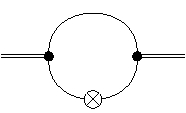
\includegraphics[width=\textwidth]{figs/TikZ/fermion_contribution}
 	\subcaption{Fermions.}
 \end{subfigure}
 \hfill
 \begin{subfigure}{0.3\textwidth} 
 	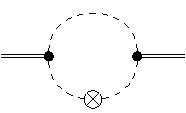
\includegraphics[width=\textwidth]{figs/TikZ/scalar_contribution}
 	\subcaption{Scalars.}
 \end{subfigure} 
 \hfill
 \begin{subfigure}{0.3\textwidth} 
 	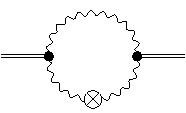
\includegraphics[width=\textwidth]{figs/TikZ/gauge_field_contribution}
 	\subcaption{Gauge Fields.}
 \end{subfigure} 
 \hfill
 \caption{Different matter contributions to the graviton anomalous dimension $\eta_h$.}	
 \end{figure}
 
 \blindtext
 
  \begin{figure}[H]
 \centering
 \hfill
 \begin{subfigure}{0.3\textwidth} 
	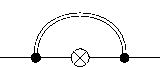
\includegraphics[width=\textwidth]{figs/TikZ/graviton_fluctuations1}
 \end{subfigure}
 \hfill
 \begin{subfigure}{0.3\textwidth}
 \vspace{-3.5pt}
 	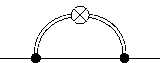
\includegraphics[width=\textwidth]{figs/TikZ/graviton_fluctuations2}
 \end{subfigure} 
 \hfill
 \begin{subfigure}{0.3\textwidth} 
 	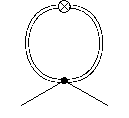
\includegraphics[scale = 1.5]{figs/TikZ/graviton_fluctuations3}
 \end{subfigure} 
 \hfill
 \caption{Contributing diagrams to the fermion anomalous dimension $\eta_D$. Analogous contributions arise for external scalars and gauge fields to $\eta_S$ and $\eta_V$.} 	
 \end{figure}